Se realizó la simlación del problema para el rango de frecuencias $\SI{80}{\mega\hertz} < f < \SI{480}{\mega\hertz}$ de a pasos de $\SI{80}{\mega\hertz}$. Los diagramas de radiación en \texttt{2D} y \texttt{3D} se muestran en las siguientes figuras.

\begin{figure}[H]
	\begin{subfigure}{0.5\textwidth}
		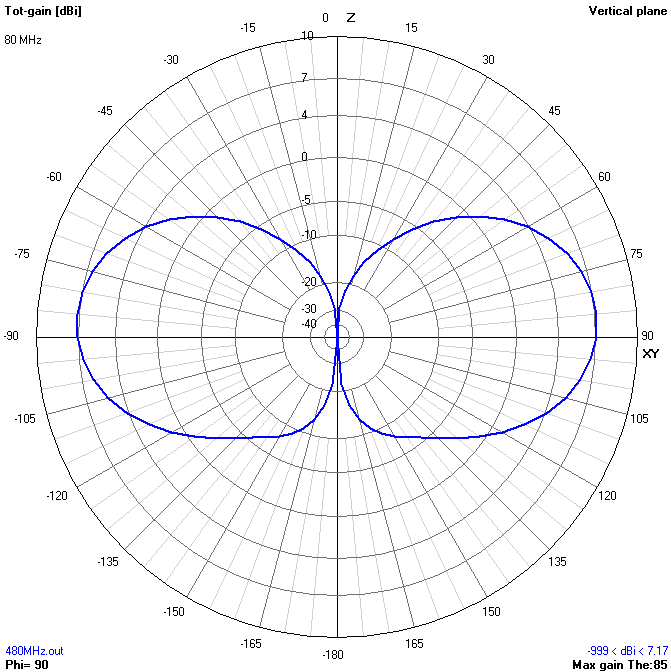
\includegraphics[scale=0.43]{imagenes/2D_80MHz.png}
	\end{subfigure}	
	\quad
	\begin{subfigure}{0.5\textwidth}
		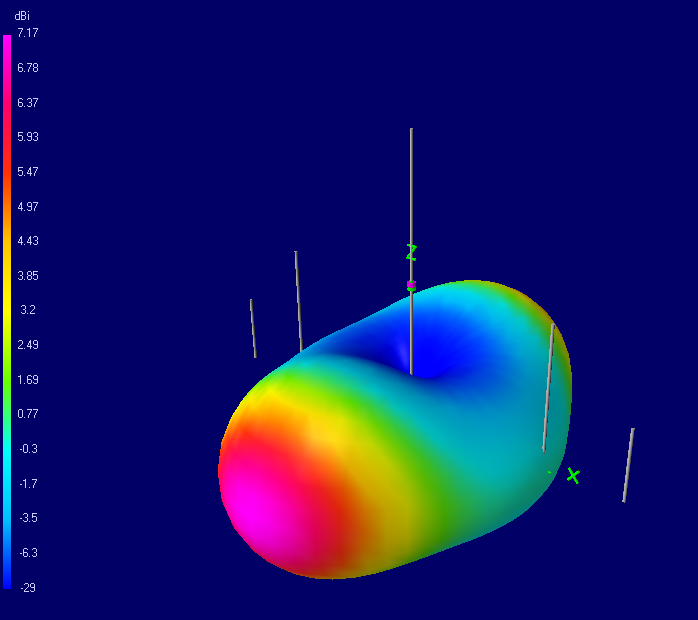
\includegraphics[scale=0.43]{imagenes/3D_80MHz.png}
	\end{subfigure}
	\caption{$f=\SI{80}{\mega\hertz}$}
	\label{fig.radiacion_80M}
\end{figure}


\begin{figure}[H]
	\begin{subfigure}{0.5\textwidth}
		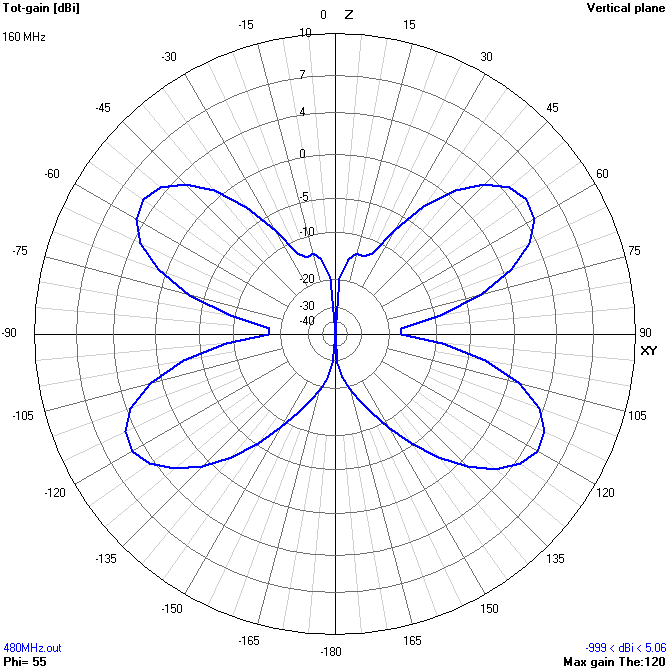
\includegraphics[scale=0.43]{imagenes/2D_160MHz.png}
	\end{subfigure}	
	\quad
	\begin{subfigure}{0.5\textwidth}
		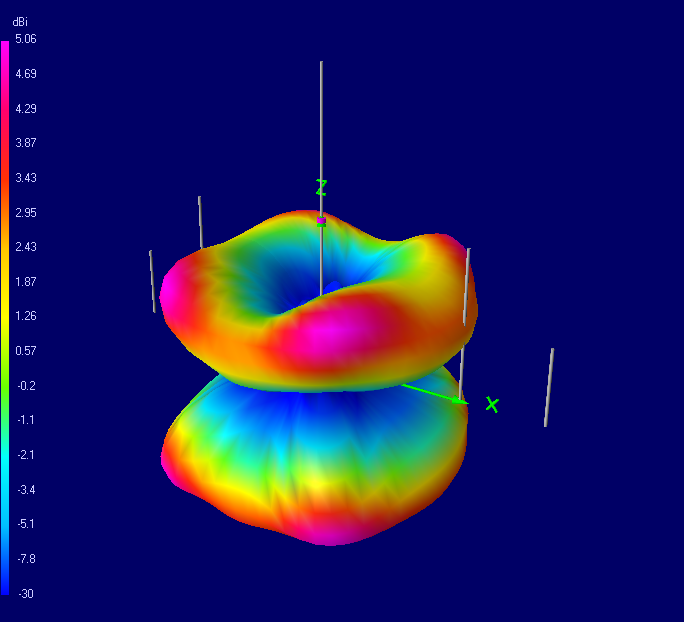
\includegraphics[scale=0.43]{imagenes/3D_160MHz.png}
	\end{subfigure}
	\caption{$f=\SI{160}{\mega\hertz}$}
	\label{fig.radiacion_160M}
\end{figure}


\begin{figure}[H]
	\begin{subfigure}{0.5\textwidth}
		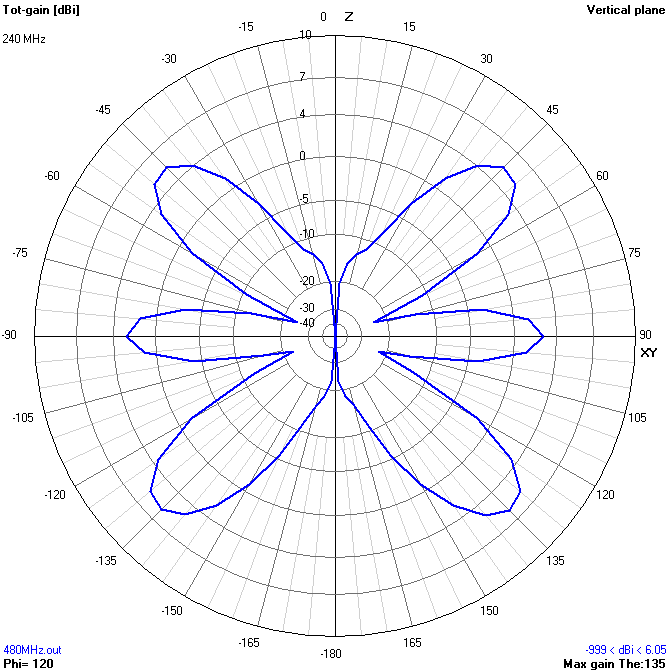
\includegraphics[scale=0.43]{imagenes/2D_240MHz.png}
	\end{subfigure}	
	\quad
	\begin{subfigure}{0.5\textwidth}
		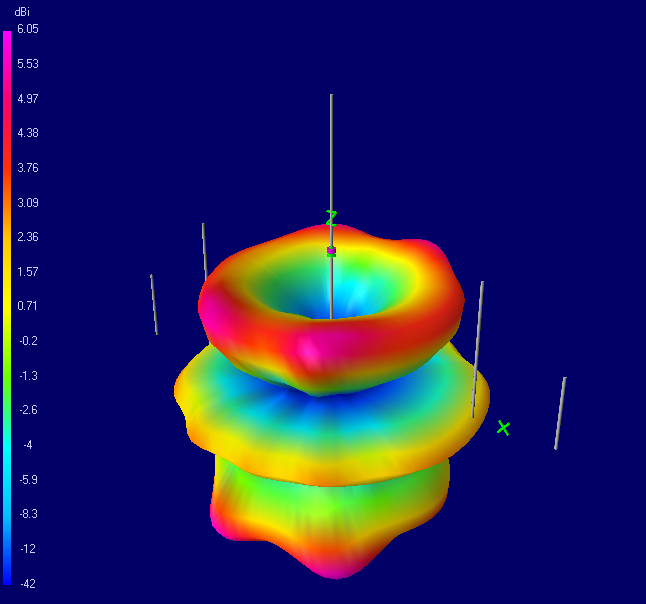
\includegraphics[scale=0.43]{imagenes/3D_240MHz.png}
	\end{subfigure}
	\caption{$f=\SI{240}{\mega\hertz}$}
	\label{fig.radiacion_240M}
\end{figure}


\begin{figure}[H]
	\begin{subfigure}{0.5\textwidth}
		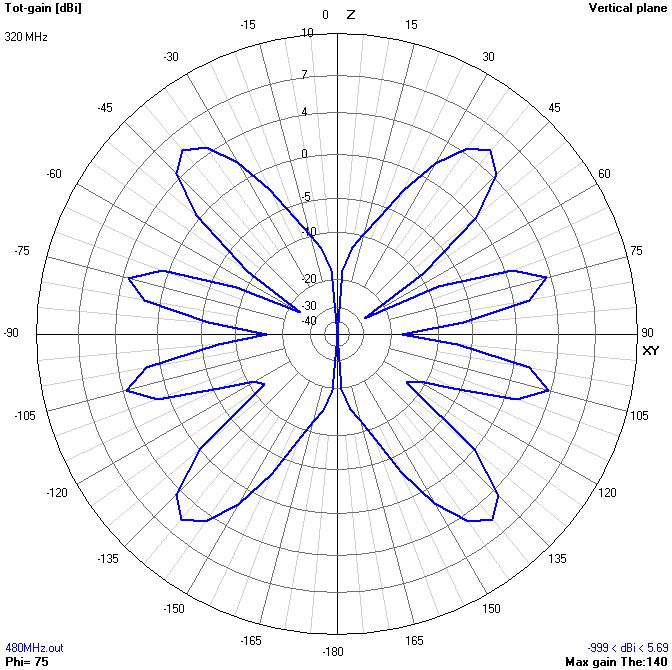
\includegraphics[scale=0.43]{imagenes/2D_320MHz.png}
	\end{subfigure}	
	\quad
	\begin{subfigure}{0.5\textwidth}
		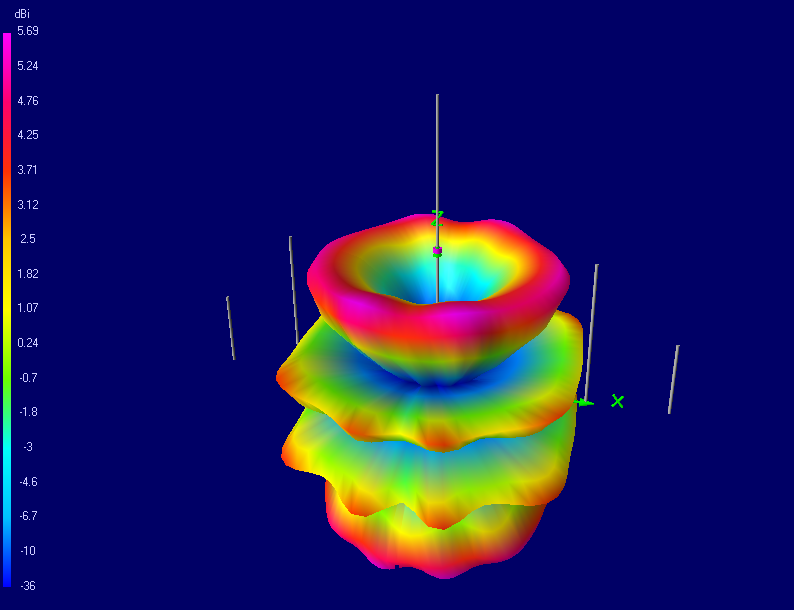
\includegraphics[scale=0.43]{imagenes/3D_320MHz.png}
	\end{subfigure}
	\caption{$f=\SI{320}{\mega\hertz}$.}
	\label{fig.radiacion_320M}
\end{figure}


\begin{figure}[H]
	\begin{subfigure}{0.5\textwidth}
		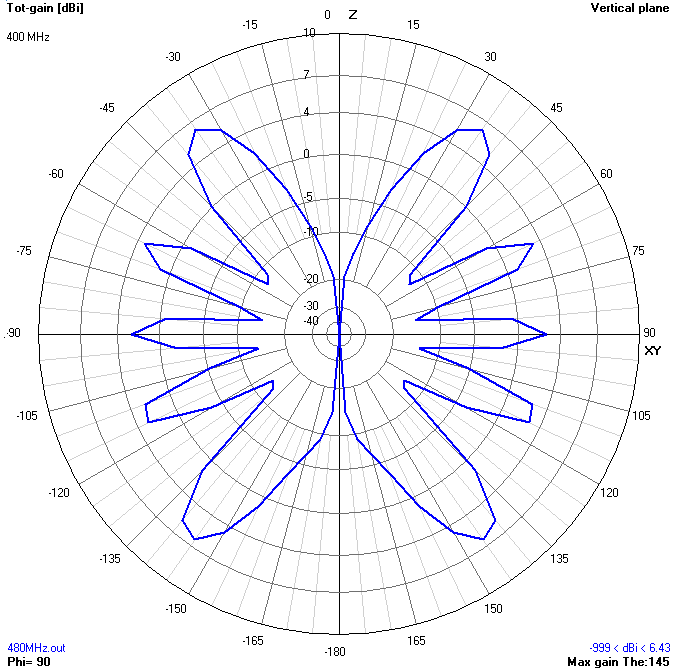
\includegraphics[scale=0.43]{imagenes/2D_400MHz.png}
	\end{subfigure}	
	\quad
	\begin{subfigure}{0.5\textwidth}
		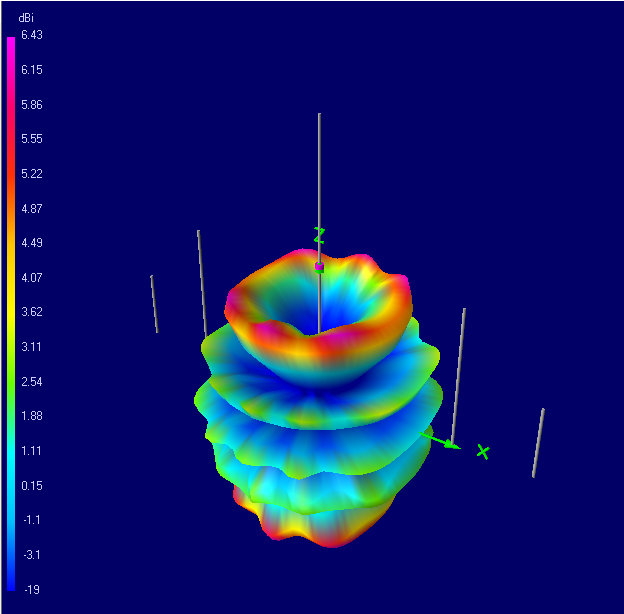
\includegraphics[scale=0.43]{imagenes/3D_400MHz.png}
	\end{subfigure}
	\caption{$f=\SI{400}{\mega\hertz}$.}
	\label{fig.radiacion_400M}
\end{figure}


\begin{figure}[H]
	\begin{subfigure}{0.5\textwidth}
		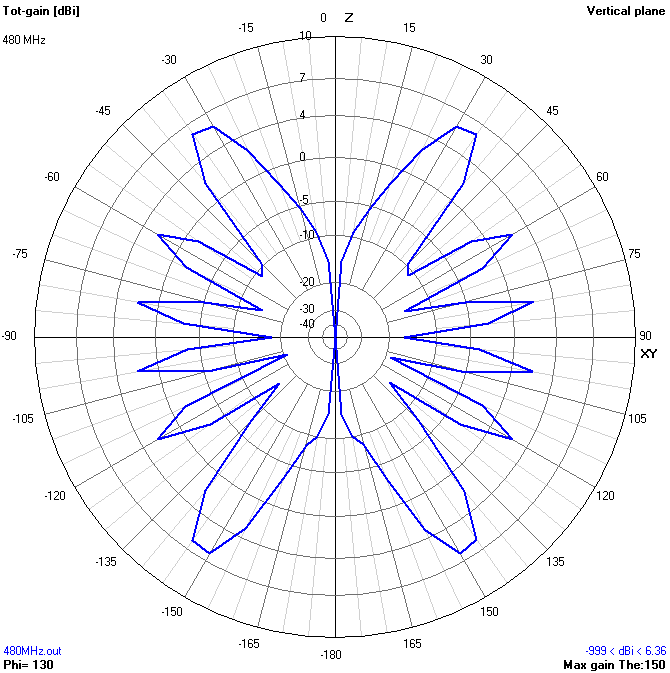
\includegraphics[scale=0.43]{imagenes/2D_480MHz.png}
	\end{subfigure}	
	\quad
	\begin{subfigure}{0.5\textwidth}
		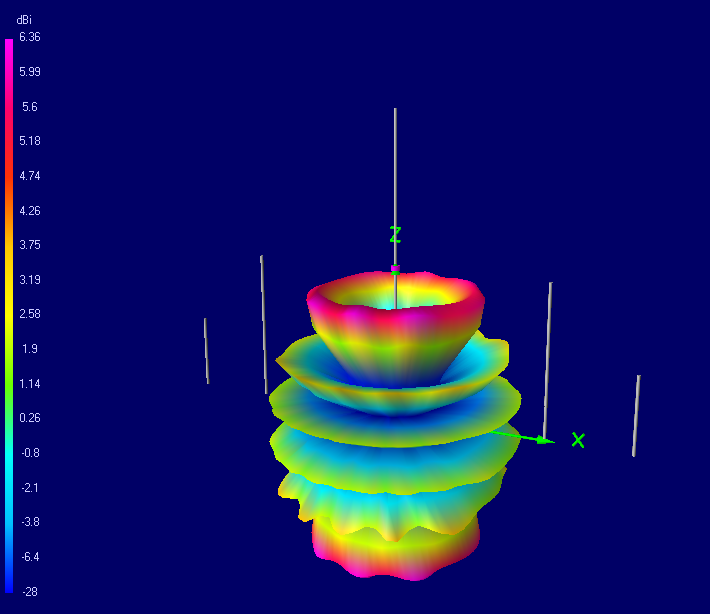
\includegraphics[scale=0.43]{imagenes/3D_480MHz.png}
	\end{subfigure}
	\caption{$f=\SI{480}{\mega\hertz}$.}
	\label{fig.radiacion_480M}
\end{figure}	


Para una frecuencia de \SI{80}{\mega\hertz} se observa la formación de dos lóbulos principales en la dirección $y$ con sentidos opuestos. En dichas direcciones se produce la máxima radiación. No hay presencia de lóbulos secundarios.
Según la figura \ref{fig.radiacion_160M} la máxima radiación se produce en ocho direcciones, tampoco se aprecian lóbulos secundarios.
A partir de la frecuencia $\SI{240}{\mega\hertz}$ hasta $\SI{480}{\mega\hertz}$ se observa que la cantidad de lóbulos principales se mantiene, mientras que aumenta la cantidad de lóbulos secundarios resultado de la interferencia entre los distintos elementos que componen la antena. La dirección de radiación a frecuencias altas es predominante en la dirección $z$. Los lóbulos secundarios irradian potencia en direcciones no controladas, que pueden dar lugar a interferencias indeseadas. Al aumentar la frecuencia la aparición de lóbulos secundarios altera la dirección y módulo de radiación. 



